\documentclass{article}
\usepackage[utf8]{inputenc}
\usepackage[margin = 0.8in]{geometry}
\usepackage{graphicx}
\usepackage{amsmath, amssymb}
\usepackage{caption}
\usepackage{subcaption}
\usepackage{multirow}
\usepackage{multicol}
\usepackage{booktabs}
\setlength{\columnsep}{.75cm}
\usepackage{float}
%\usepackage[parfill]{parskip}. %to not indent paragraph
\renewcommand\refname{References}

\title{RBE502 - Project- Group F}
\author{Keith Chester, Bob DeMont, Sean Hart}         %Enter your name and last name
\date{Due date: November  9, 2021}

\begin{document}
\maketitle
\section*{Situation/Problem}
The mission is defense of a designated airspace.  Our quadrotor is assigned to monitor a limited airspace, launch if an unidentified UAV enters that airspace, capture the bogey and return to base without leaving the airspace.  If the bogey leaves the airspace before being captured, our quadrotor should return to base.  When captured the bogey should be assumed to generate external forces on our UAV. The figure below depicts the scenario.
\begin{figure}[H]
    \centering
    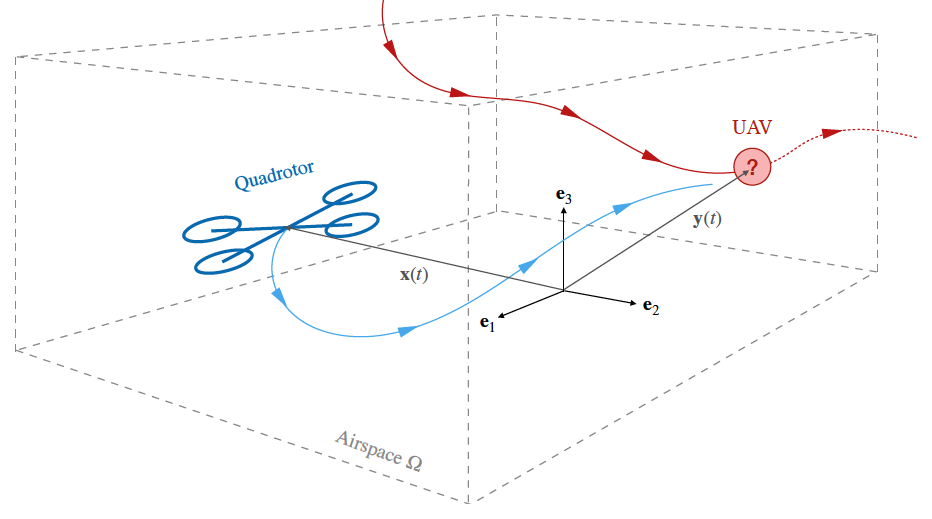
\includegraphics[width = 1.0\textwidth]{figures/ProjProbStmt.png}
     \label{fig:prob}
\end{figure}

%\begin{multicols}{2}
\section*{Materials and Methods}
Coordinate frames are identified for the reference/inertial frame $E={e_1, e_2, e_3}$ at the center bottom of the airspace and the body frame $C={c_1, c_2, c_3}$.  All rotors are equidistant from the center of mas and in the same $c_1-c_2 $ plane as the body center of mass.

The external forces and moments on the system are represented by $\boldsymbol{r}$ and $\boldsymbol{n}$, where $\boldsymbol{r} = r_1 c_1 + r_2 c_2 + r_3 c_3$ and $\boldsymbol{n} = n_1 c_1 + n_2 c_2 + n_3 c_3$ directly applied to the center of mass. We are assuming that the torque of the rotor is proportionaly related to the input thrust via the constant $\sigma>0$, for $\tau_i = \sigma u_i$. We will be utilizing $\boldsymbol{I}$ as our inertial matrix, where:

\begin{equation}
    \boldsymbol{I} = \begin{bmatrix}
        I_x & 0 & 0 \\
        0 & I_y & 0 \\
        0 & 0 & I_z \\
    \end{bmatrix}
\end{equation}
where $I_x, I_y $ and $I_z$ represent the mass moments of inertia about $c_1, c_2 $ and $c_3$ respectively.  
%Table 

\begin{table}[]
\begin{centering}
\begin{tabular}{|cccc|}
\hline
Parameter & Value & Units  & Description  \\
\hline
 $l$  &  .02& m & Distance from center of mass to center of each rotor  \\
 $m$& .5 & kg &Total mass of quadrotor   \\
 $I_{x}$ & 1.24 kgm$^2 $ & s  & Mass moment of inertia about $c_1$ axis \\
 $I_{y}$ & 1.24 kgm$^2 $ & s  & Mass moment of inertia about $c_2$ axis \\
 $I_{z}$ & 1.24 kgm$^2 $ & s  & Mass moment of inertia about $c_3$ axis \\
$ g$ &9.81 & m/s$^2$ & Gravitational acceleration\\
$\sigma\ $& .01 & m & Proportionality constant relating $u_i $ to $\tau_i$\\
\hline
\end{tabular}
\caption{Quadrotor Parameters}
\label{tab:Qparams}
\end{centering}
\end{table}

We have also had established for us that there exists a rotation matrix - $R_{C/E}$ - which rotates from frame $C$ to frame $E$. This rotaton matrix is the result of a Euler angle $z-y-x$ rotation along $\phi$,  $\theta$, and $\psi$, respectively. This rotation matrix is such that:

\begin{equation}
    R_{C/E} =
    \begin{bmatrix}
        \cos \left(\psi \right)\,\cos \left(\theta \right) & \cos \left(\psi \right)\,\sin \left(\phi \right)\,\sin \left(\theta \right)-\cos \left(\phi \right)\,\sin \left(\psi \right) & \sin \left(\phi \right)\,\sin \left(\psi \right)+\cos \left(\phi \right)\,\cos \left(\psi \right)\,\sin \left(\theta \right)\\
        \cos \left(\theta \right)\,\sin \left(\psi \right) & \cos \left(\phi \right)\,\cos \left(\psi \right)+\sin \left(\phi \right)\,\sin \left(\psi \right)\,\sin \left(\theta \right) & \cos \left(\phi \right)\,\sin \left(\psi \right)\,\sin \left(\theta \right)-\cos \left(\psi \right)\,\sin \left(\phi \right)\\
        -\sin \left(\theta \right) & \cos \left(\theta \right)\,\sin \left(\phi \right) & \cos \left(\phi \right)\,\cos \left(\theta \right)
    \end{bmatrix}
\end{equation}
And 
\begin{equation}
    T^{-1} = \begin{bmatrix}
        1 & \sin{\phi} \tan{\theta} & \cos{\phi}\tan{theta} \\
        0 & \cos{\phi} & -\sin{\phi} \\
        0 & \frac{\sin{\phi}}{\cos{\theta}} & \frac{\cos{\phi}}{\theta}
    \end{bmatrix}
\end{equation}

\section*{Results}
\section*{Discussion}



\label{References}
\bibliographystyle{abbrv}
\begin{thebibliography}{10}
\bibitem{AHM}
Faraz Ahmad, Pushpendra Kumar, Anamika Bhandari, Pravin P. Patil.
Simulation of the Quadcopter Dynamics with LQR based Control.
Materials Today: Proceedings,Volume 24, Part 2, 2020, Pages 326-332,
ISSN 2214-7853.
https://doi.org/10.1016/j.matpr.2020.04.282.
\bibitem{JKim}
Jinho Kim, S. Andrew Gadsden, Stephen A . Wilkerson.
"A Comprehensive Survey of Control Strategies for Autonomus Quadrotors".
arXiv:2005.09858v1.
20 May 2020.
\bibitem{MAD}
Madani, T, and A Benallegue.
“Backstepping Control for a Quadrotor Helicopter.” 
2006 IEEE/RSJ International Conference on Intelligent Robots and Systems. 
IEEE, 2006. 3255–3260. Web.
\bibitem{QIAO}
Jing Qiao, Zhixiang Liu, Youmin Zhang. "Payload Dropping Control of an Unmanned Quadrotor Helicopter Based on Backstepping Controller".
MATEC Web Conf., 277 (2019) 01004.
DOI: https://doi.org/10.1051/matecconf/201927701004.
\bibitem{ZHEN}
Jia, Zhenyue and Yu, Jianqiao and Ai, Xiaolin.
"Integral Backstepping Control for Quadrotor Helicopters".
Association for Computing Machinery.
2017.
DOI:https://doi-org./10.1145/3057039.3057052
\bibitem{LEE}
Daewon Lee, H JIN Kim, Shankar Sastry.  
Feedback Linearization vs Adaptive Sliding Mode Control for a Quadrotor Helicopter. 
International Journal of Control, Automation, and Systems (2009). DOI 10.1007/s 12555-009-0311-8.
\end{thebibliography}
%\end{multicols}
\end{document}
